\documentclass[a4paper, 10pt, final, garamond]{book}
\usepackage{cours-preambule}
\graphicspath{{./figures/}}

\makeatletter
\renewcommand{\@chapapp}{Contr\^ole de connaissances}
\makeatother

% \toggletrue{student}
% \HideSolutionstrue

\begin{document}
\setcounter{chapter}{5}

\chapter{Électrocinétique~: ressort amorti\ifstudent{ (13')}}

\begin{enumerate}[label=\sqenumi, leftmargin=10pt]
	\nitem{10}
	\noindent
	\begin{minipage}[t]{.65\linewidth}
		On suppose le système mécanique suivant, constitué du point M de masse $m$
		accroché à un ressort idéal mais subissant des frottements fluides. On
		travaille dans le référentiel $\Rc\ind{sol}(O',x,y,t)$ supposé galiléen,
		avec le repère $(\Or', \ux, \uy)$. On repère la masse par rapport à sa
		position d'équilibre~: $x (t) = \ell(t) - \ell_0$. On suppose le ressort
		initialement détendu tel que $x (0) = x_0 > 0$, lâché sans vitesse initiale.
	\end{minipage}
	\hfill
	\begin{minipage}[t]{.32\linewidth}
		~
		\vspace{-35pt}
		\begin{center}
			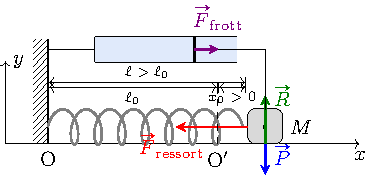
\includegraphics[width=\linewidth]{ressort_amorti}
			% \vspace*{-10pt}
			\captionof{figure}{}
		\end{center}
	\end{minipage}
	Effectuer un bilan des forces puis déterminer l'équation différentielle sous
	forme canonique de $x (t)$ pour $t \geq 0$. Déterminer les expressions de
	$\w_0$ et $Q$, résoudre l'équation différentielle pour un régime
	pseudo-périodique.
	\smallbreak
	Exprimer la période $T$ des oscillations amorties en fonction de la période
	$T_0$ des oscillations harmoniques, donner \textit{sans démonstration}
	l'approximation de $t_{95}$ et \textbf{tracer la solution}, avec $Q \approx
		3$.
	\smallbreak
	\begin{isd}[sidebyside align=top]
		\wsw{
			\begin{itemize}[label=$\diamond$, leftmargin=10pt]
				\bitem{Bilan des forces~:}
				\[
					\begin{array}{ll}
						\textbf{Poids}               & \Pf = m\gf = -mg \uy \\
						\textbf{Réaction normale}    & \Rf = R\uy           \\
						\textbf{Force de rappel}     & \Ff_r = -kx (t)\ux   \\
						\textbf{Force de frottement} & \Ff_{f} = -\alpha\vf
					\end{array}
				\]
			\end{itemize}
			Avec le PFD~:
			\begin{DispWithArrows*}[fleqn, mathindent=0pt, groups]
				m\af &= \Pf + \vv{R} + \Ff_{r} + \Ff_{f}
				\Arrow{Dvlp$^{\xul{\rm t}}$}
				\\
				\Lra m\left(
				\begin{array}{c}
						\dv[2]{x}{t} \\
						0
					\end{array}
				\right)
				&=
				\left(
				\begin{array}{c}
						-kx -\alpha v \\
						-mg + R
					\end{array}
				\right)
				\Arrow{$\cdot \ux$}
				\\\Ra
				m \dv[2]{x}{t} + \alpha \dv{x}{t} + kx &= 0
				\Arrow[new-group]{Forme canonique}
				\\\Lra
				\dv[2]{x}{t} + \frac{\w_0}{Q} \dv{x}{t} + \w_0{}^{2}x &= 0
			\end{DispWithArrows*}
			On détermine l'expression de $Q$ par identification~:
			\begin{align*}
				\frac{\w_0}{Q} = \frac{\alpha}{m}
				 & \Lra
				\frac{1}{Q}\sqrt{\frac{k}{m}} = \frac{\alpha}{m}
				\\\Lra
				Q = \frac{m}{\alpha} \sqrt{\frac{k}{m}}
				 & \Lra
				\boxed{Q = \frac{\sqrt{km}}{\alpha}}
			\end{align*}
			On part de l'équation caractéristique~:
			\begin{gather*}
				r^{2} + \frac{\w_0}{Q}r + \w_0{}^{2} = 0
				\Ra
				\boxed{\Delta = \frac{\w_0{}^{2}}{Q^{2}}\left( 1-4Q^{2} \right) < 0}
			\end{gather*}
			\begin{DispWithArrows*}[fleqn, mathindent=5pt]
				\Ra
				r_\pm & = \frac{-\frac{\w_0}{Q} \pm \jj\sqrt{-\D}}{2}
				\Arrow{On injecte $\Delta$\\et extrait $\frac{\w_0}{Q}$}
				\\\Lra
				r_\pm &= - \frac{\w_0}{2Q} \pm \jj \frac{\w_0}{2Q} \sqrt{4Q^{2}-1}
				\Arrow{$\W = \frac{\w_0}{2Q}\sqrt{4Q^{2}-1}$}
				\\\Lra
				r_\pm &= - \frac{\w_0}{2Q} \pm \jj\W
			\end{DispWithArrows*}
		}
		\tcblower
		\wsw{
			Ensuite, avec la forme générale de la solution on a
			\begin{equation*}
				x(t) = \exp \left(-\frac{\w_0}{2Q}t\right)
				\left[ A\cos(\Wt) + B\sin(\Wt) \right]
			\end{equation*}
			\begin{itemize}
				\item On trouve $A$ avec la première condition initiale~:
				      \begin{gather*}
					      x(0) = x_0 = 1 \left[ A \cdot 1 + B \cdot 0 \right] = A
					      \quad \Ra \quad \boxed{A=x_0}
				      \end{gather*}
				\item On trouve $B$ avec la seconde CI~:
				      \begin{align*}
					      \dv{x}{t}      & =
					      -\frac{\w_0}{2Q}\exp \left( -\frac{\w_0}{2Q}t \right)
					      \times
					      \left[ A\cos(\Wt) + B\sin(\Wt) \right]
					      \\
					                     & +
					      \exp \left( -\frac{\w_0}{2Q}t \right)
					      \times
					      \left[ -A\W\sin(\Wt) + B\W\cos(\Wt) \right]
					      \\\Ra
					      \dv{x}{t}\/(0) & = - \frac{\w_0}{2Q}A + \W B = 0
					      \\\Lra
					      \Aboxed{B      & = \frac{\w_0}{2Q\W}x_0
						      = \frac{x_0}{\sqrt{4Q^2-1}}}
				      \end{align*}
			\end{itemize}
			Ainsi, on trouve bien
			\[
				\boxed{
					x(t) = x_0\exp \left( -\frac{\w_0}{2Q}t \right)\times
					\left[
						\cos(\Wt) + \frac{1}{\sqrt{4Q^2 - 1}}\sin(\Wt)
						\right]
				}
			\]
			\begin{equation*}
				\Ra
				\boxed{
					T =
					\frac{2\pi}{\W} =
					T_0 \frac{2Q}{\sqrt{4Q^{2} - 1}}
				}
				\qet
				\boxed{t_{95} \approx QT_0}
			\end{equation*}
		}
		\begin{center}
			\switch{
				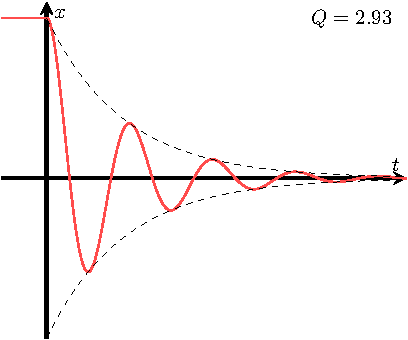
\includegraphics[width=.7\linewidth, draft=true]{carac-ra-3}
			}{
				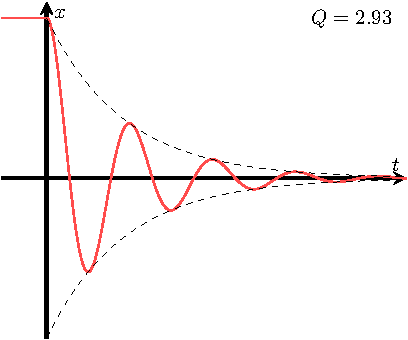
\includegraphics[width=.7\linewidth]{carac-ra-3}
			}
			\captionof{figure}{Tracé solution $Q \approx 3$.}
		\end{center}
		\vspace*{-20pt}
	\end{isd}
	\vspace*{-20pt}
\end{enumerate}

\ifstudent{
	\begin{tikzpicture}[remember picture, overlay]
		\node[anchor=north west, align=left]
		at ([shift={(1.4cm,0)}]current page.north west)
		{\\[5pt]\Large\bfseries Nom~:\\[10pt]\Large\bfseries Prénom~:};
		\node[anchor=north east, align=right]
		at ([shift={(-1.5cm,-17pt)}]current page.north east)
		{\Large\bfseries Note~:\hspace{1cm}/10};
	\end{tikzpicture}
}

\end{document}
